
 \documentclass{beamer}

\usepackage{ucs}
\usepackage[utf8x]{inputenc}
\usepackage[T1]{fontenc}
\usepackage[english]{babel}
\usepackage[retainorgcmds]{IEEEtrantools}%	IEEEeqnarray
\usepackage{mathabx}%	convolution symbol
\usepackage{multi row}
\usepackage{listings}

\usepackage{epstopdf}

\lstset{
	language=C++,
	basicstyle=\footnotesize,
	showtabs=true,
	tabsize=3,
}

%	presentation info
\title{Optimization of a Finite-Volume Method Application}

\subtitle{MPI: Implementation and Analysis}

\author{José Alves, Rui Brito}

\institute[22765, 22781]{
	Universidade do Minho
}

\date{Braga, June 2013}


%	beamer options
\usetheme{CambridgeUS}


\begin{document}%	begin presentation

\maketitle%	title slide

\begin{frame}
	\frametitle{Index}
	\tableofcontents
\end{frame}

\begin{frame}
	\frametitle{Convection-Diffusion (Recap)}
	\begin{description}
		\item [What?] Computes the heat diffusion of a fluid spreading over an area;
		\item [How?] Uses a Finite-Volume method;
		\item [Why?] Represents surface as a mesh, making each cell only dependent of its neighbours;
	\end{description}
\end{frame}

\section{Implementation}

\begin{frame}
	\frametitle{Approach}
	\begin{itemize}
		\item Mesh is shared by all processes;
		\item Work is divided among all processes;
		\item Master process gathers all data;		
	\end{itemize}
\end{frame}


\begin{frame}
	\frametitle{Problems}
	\begin{itemize}		
		\item High level of communication between processes;
		\item High level of barrier synchronization;
		\item Some balancing problems;
		\item Computed error spikes;
		\item Some of FVLib's templates are hard to serialize (locality);
		\item Sequential portion is slow;
	\end{itemize}
\end{frame}



\section{Results}

\begin{frame}
	\frametitle{Environment}
	\begin{block}{Environmental Setup}
		\begin{itemize}
			\item{SeARCH Group 101
			\begin{itemize}
				\item[-]{64-bit Intel\textregistered Xeon\texttrademark @ 3.2 GHz;}
				\item[-]{4 hardware threads per node;}
				\item[-]{16 KB L1 data cache, 2 MB L2 cache, 2 GB RAM;}
			\end{itemize}
			}			
		\end{itemize}
	\end{block}	
\end{frame}

\begin{frame}
	\frametitle{Results}
	\begin{figure}[!htp]
    \centering   
        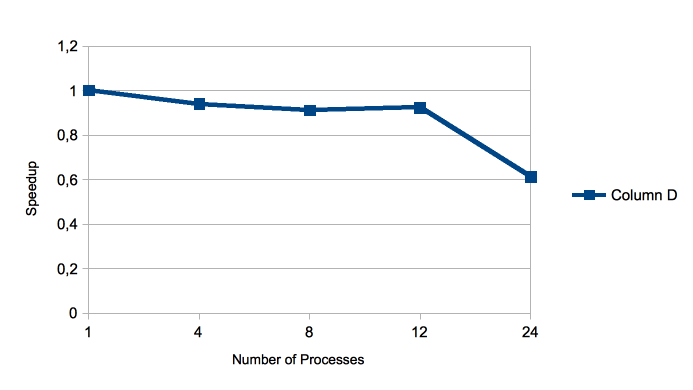
\includegraphics[width=.9\textwidth]{images/speedup.png}
        \caption{Achieved Speedups}    
\end{figure}
\end{frame}

\begin{frame}
	\frametitle{Results}
	\begin{figure}[!htp]
    \centering   
        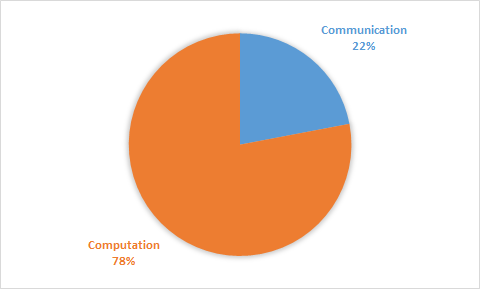
\includegraphics[width=.9\textwidth]{images/com.png}
        \caption{Communication/Computation Ratio}    
\end{figure}
\end{frame}


\section{Conclusions}

\begin{frame}
	\frametitle{Conclusions}
	\begin{itemize}
		\item Excessive communication hinders performance in MPI;
		\item FVLib's templates were a problem;
		\item Further optimization would be difficult;
	\end{itemize}	
\end{frame}

\section{Roadmap}

\begin{frame}
\frametitle{Roadmap}
	\begin{center}	
	\begin{itemize}		
		\item Converting structures to SOA;
		\item Optimize for OpenMP;
		\item Finally try a CUDA implementation;
	\end{itemize}
	\end{center}
\end{frame}

\begin{frame}
\titlepage
	\begin{center}
		\Huge\bfseries
		- ? -
	\end{center}
\end{frame}

\end{document}%	end presentation